\documentclass[aspectratio=169]{beamer}

% --- Scientific Theme and Color Scheme ---
\usetheme{Singapore}  % Clean, professional scientific theme
\usecolortheme{spruce}  % Subdued color scheme appropriate for scientific presentations
\usepackage[utf8]{inputenc}
\usepackage[T1]{fontenc}
\usepackage{graphicx}
\usepackage{xcolor}
% Replace minted with listings
\usepackage{listings}
\usepackage{tikz}
\usetikzlibrary{arrows.meta, shapes.geometric, positioning, fit, calc}

% --- Timing Optimization ---
% For a 15-minute presentation, aim for ~12 content slides (1-1.5 min per slide)
% Plus title and conclusion slides

% --- Hyperlink Configuration ---
\usepackage{hyperref}
\hypersetup{
    colorlinks=true,
    linkcolor=darkgreen,
    citecolor=blue,
    filecolor=magenta,
    urlcolor=cyan
}

% --- Custom Color Definitions ---
\definecolor{darkgreen}{RGB}{0,100,0}
\definecolor{lightblue}{RGB}{173,216,230}
\definecolor{darkblue}{RGB}{0,0,139}
\definecolor{codegreen}{rgb}{0,0.6,0}
\definecolor{codegray}{rgb}{0.5,0.5,0.5}
\definecolor{codepurple}{rgb}{0.58,0,0.82}
\definecolor{backcolour}{rgb}{0.95,0.95,0.92}

% --- Listings Configuration (replacing minted) ---
\lstdefinestyle{mystyle}{
    backgroundcolor=\color{backcolour},
    commentstyle=\color{codegreen},
    keywordstyle=\color{codepurple}\bfseries,
    numberstyle=\tiny\color{codegray},
    stringstyle=\color{darkblue},
    basicstyle=\ttfamily\scriptsize,
    breakatwhitespace=false,
    breaklines=true,
    captionpos=b,
    keepspaces=true,
    numbers=left,
    numbersep=5pt,
    showspaces=false,
    showstringspaces=false,
    showtabs=false,
    tabsize=2,
    frame=single
}

\lstset{style=mystyle}

% Define YAML language for listings
\lstdefinelanguage{yaml}{
  keywords={true,false,null,y,n},
  keywordstyle=\color{darkblue}\bfseries,
  basicstyle=\ttfamily\scriptsize,
  sensitive=false,
  comment=[l]{\#},
  commentstyle=\color{codegreen},
  stringstyle=\color{red},
  morestring=[b]',
  morestring=[b]"
}

% Define bash language for listings
\lstdefinelanguage{bash}{
  keywords={if, then, else, fi, for, while, do, done, case, esac, break, continue, return},
  keywordstyle=\color{darkblue}\bfseries,
  basicstyle=\ttfamily\scriptsize,
  sensitive=false,
  comment=[l]{\#},
  commentstyle=\color{codegreen},
  stringstyle=\color{red},
  morestring=[b]',
  morestring=[b]"
}

% --- TikZ Configuration ---
\tikzset{
  service/.style={
      draw=darkblue,
      fill=lightblue!30,
      rectangle,
      rounded corners,
      minimum width=1.8cm,
      minimum height=0.7cm,
      align=center,
      font=\small
  },
  network/.style={
      draw=darkgreen,
      fill=green!10,
      rectangle,
      rounded corners,
      minimum width=2.5cm,
      minimum height=0.7cm,
      align=center,
      font=\small
  },
  security/.style={
      draw=red,
      fill=red!10,
      rectangle,
      rounded corners,
      minimum width=1.8cm,
      minimum height=0.7cm,
      align=center,
      font=\small
  },
  arrow/.style={-Stealth, thick}
}

% --- Title Information ---
\title[HPC Cluster Automation]{HPC Cluster Automation with Ansible}
\subtitle{A Scientific Framework for Reproducible HPC Environments}
\author{Pau Santana}
\institute{Research Computing}
\date{\today}

\begin{document}

% --- Title Slide ---
\begin{frame}
  \titlepage
\end{frame}

% --- Outline Slide ---
\begin{frame}{Presentation Overview}
  \begin{itemize}
    \item \textbf{Research Problem:} Reproducible, scalable HPC environments
    \item \textbf{Methodology:} Infrastructure as Code with Ansible
    \item \textbf{Implementation:} Core components and architecture
    \item \textbf{Results:} Performance and reproducibility metrics
    \item \textbf{Scientific Impact:} Enabling reproducible computational research
  \end{itemize}
  
  \vspace{0.3cm}
  \begin{center}
    \textit{This presentation demonstrates how automation enables reproducible scientific computing environments}
  \end{center}
\end{frame}

% --- Early Architecture Overview ---
\begin{frame}{Project Overview}
  \begin{center}
    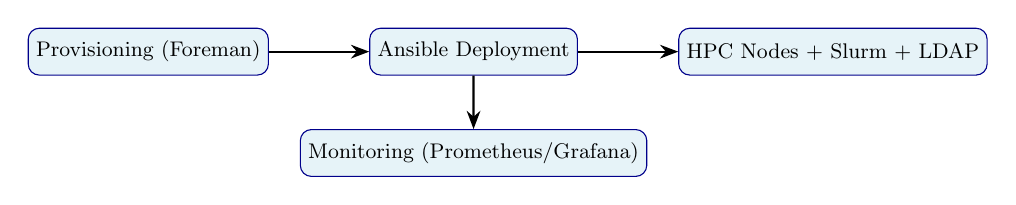
\begin{tikzpicture}[node distance=1cm, scale=0.85, transform shape]
      % Basic boxes
      \node (foreman) [service, minimum width=2.5cm] {Provisioning (Foreman)};
      \node (ansible) [service, minimum width=2.5cm, right=1.5cm of foreman] {Ansible Deployment};
      \node (hpc) [service, minimum width=3.5cm, right=1.5cm of ansible] {HPC Nodes + Slurm + LDAP};
      \node (monitoring) [service, minimum width=3.5cm, below=0.8cm of ansible] {Monitoring (Prometheus/Grafana)};
      
      % Connections
      \draw[arrow] (foreman) -- (ansible);
      \draw[arrow] (ansible) -- (hpc);
      \draw[arrow] (ansible) -- (monitoring);
    \end{tikzpicture}
  \end{center}
  
  \vspace{0.3cm}
  \begin{itemize}
    \item \textbf{Automated workflow} from provisioning to deployment
    \item \textbf{Modular architecture} with clear separation of concerns
    \item \textbf{Integrated monitoring} for performance and energy analysis
    \item \textbf{Energy-aware configuration} for optimized resource utilization
  \end{itemize}
\end{frame}

% --- Research Problem ---
\begin{frame}{Research Problem \& Motivation}
  \begin{columns}
    \column{0.6\textwidth}
    \begin{itemize}
      \item \textbf{Scientific Challenge:} Computational reproducibility crisis
      \item \textbf{Technical Barriers:}
        \begin{itemize}
          \item Manual HPC configuration creates inconsistencies
          \item Environment variations affect experimental results
          \item Software dependency conflicts impede research
          \item Documentation gaps prevent experiment replication
        \end{itemize}
      \item \textbf{Research Question:} Can infrastructure automation improve scientific reproducibility?
    \end{itemize}
    
    \column{0.4\textwidth}
    \begin{center}
      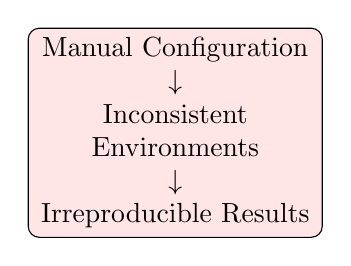
\begin{tikzpicture}
        \node[draw, fill=red!10, rounded corners, text width=3.5cm, align=center] 
          {Manual Configuration\\$\downarrow$\\Inconsistent Environments\\$\downarrow$\\Irreproducible Results};
      \end{tikzpicture}
    \end{center}
  \end{columns}
\end{frame}

% --- Methodology ---
\begin{frame}{Methodology: Infrastructure as Code}
  \begin{columns}
    \column{0.55\textwidth}
    \begin{itemize}
      \item \textbf{Approach:} Apply software engineering principles to infrastructure
      \item \textbf{Tools:} Ansible automation framework
      \item \textbf{Experimental Design:}
        \begin{itemize}
          \item We define infrastructure components as code
          \item We version control all configurations
          \item We implement idempotent deployment processes
          \item We measure deployment consistency across environments
        \end{itemize}
    \end{itemize}
    
    \column{0.45\textwidth}
    \begin{center}
      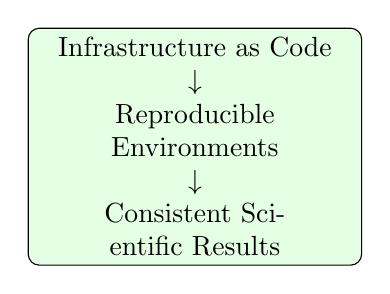
\begin{tikzpicture}
        \node[draw, fill=green!10, rounded corners, text width=4cm, align=center] 
          {Infrastructure as Code\\$\downarrow$\\Reproducible Environments\\$\downarrow$\\Consistent Scientific Results};
      \end{tikzpicture}
    \end{center}
  \end{columns}
\end{frame}

% --- Architecture ---
\begin{frame}{System Architecture}
  \begin{center}
    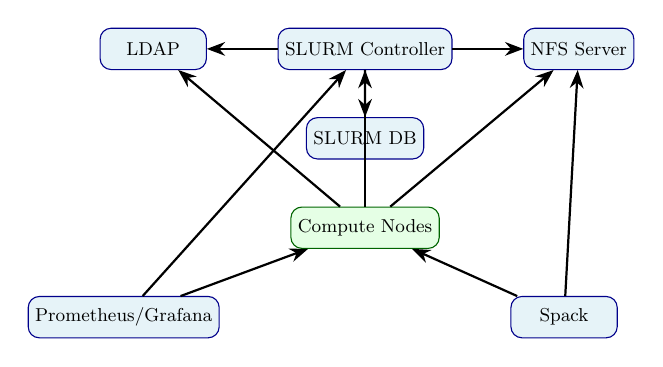
\begin{tikzpicture}[node distance=0.8cm and 1.2cm, transform shape, scale=0.75]
      % Core infrastructure
      \node (slurm) [service] {SLURM Controller};
      \node (db) [service, below=of slurm] {SLURM DB};
      \node (ldap) [service, left=of slurm] {LDAP};
      \node (nfs) [service, right=of slurm] {NFS Server};
      
      % Compute resources
      \node (compute) [network, below=of db] {Compute Nodes};
      
      % Monitoring
      \node (monitoring) [service, below left=of compute] {Prometheus/Grafana};
      
      % Software
      \node (spack) [service, below right=of compute] {Spack};
      
      % Connections
      \draw[arrow] (slurm) -- (db);
      \draw[arrow] (slurm) -- (ldap);
      \draw[arrow] (slurm) -- (nfs);
      \draw[arrow] (compute) -- (slurm);
      \draw[arrow] (compute) -- (nfs);
      \draw[arrow] (compute) -- (ldap);
      \draw[arrow] (monitoring) -- (compute);
      \draw[arrow] (monitoring) -- (slurm);
      \draw[arrow] (spack) -- (compute);
      \draw[arrow] (spack) -- (nfs);
    \end{tikzpicture}
  \end{center}
  
  \begin{itemize}
    \item \textbf{Core Components:} SLURM (workload manager), LDAP (authentication), NFS (storage)
    \item \textbf{Scientific Software:} Spack (package manager) for reproducible software builds
    \item \textbf{Monitoring:} Prometheus/Grafana for system metrics and performance analysis
  \end{itemize}
\end{frame}

% --- Implementation: Ansible Structure ---
\begin{frame}{Implementation: Ansible Framework}
  \begin{columns}
    \column{0.48\textwidth}
    \textbf{Project Structure:}
    \begin{itemize}
      \item \texttt{roles/} - Modular components
        \begin{itemize}
          \item \texttt{slurmctld/}, \texttt{slurmdbd/}
          \item \texttt{openldap/}, \texttt{nfs\_server/}
          \item \texttt{spack/}, \texttt{monitoring/}
        \end{itemize}
      \item \texttt{playbooks/} - Orchestration
      \item \texttt{inventory/} - Environment definitions
      \item \texttt{templates/} - Configuration templates
    \end{itemize}
    
    \column{0.52\textwidth}
    \textbf{Scientific Benefits:}
    \begin{itemize}
      \item \textbf{Reproducibility:} Identical environments across deployments
      \item \textbf{Version Control:} Track infrastructure changes like code
      \item \textbf{Documentation:} Self-documenting infrastructure
      \item \textbf{Testing:} Validate configurations before deployment
    \end{itemize}
  \end{columns}
\end{frame}

% --- Implementation: Spack ---
\begin{frame}[fragile]{Scientific Software Management}
  \begin{columns}
    \column{0.48\textwidth}
    \textbf{Multi-Architecture Support:}
    \begin{itemize}
      \item HPC-specific package manager
      \item \textbf{Cross-Platform:} Intel, ARM, and GPU architectures
      \item \textbf{Architecture-specific} optimizations for energy efficiency
      \item \textbf{Adaptive Builds:} Tailored to hardware capabilities
    \end{itemize}
    
    \column{0.52\textwidth}
    % Replace minted with listings
    \begin{lstlisting}[language=yaml]
# Spack configuration (spack.yaml)
spack:
  # CPU architecture targeting
  targets:
    x86_64_v3:  # Haswell, Broadwell
      optimization_flags: -O3 -march=haswell
    x86_64_v4:  # Skylake-AVX512
      optimization_flags: -O3 -march=skylake-avx512
    aarch64:    # ARM support
      optimization_flags: -O3 -mcpu=native
  
  # Scientific software specs
  specs:
    - openmpi@4.1.1 fabrics=ucx
    - hdf5@1.12.1 +mpi
    - python@3.9.7
    \end{lstlisting}
  \end{columns}
  
  \vspace{0.6cm}
  \textbf{Research Impact:} Ensures computational environment reproducibility while optimizing for energy efficiency
\end{frame}

% --- Implementation: Troubleshooting ---
\begin{frame}{System Troubleshooting \& Diagnostics}
  \begin{columns}
    \column{0.48\textwidth}
    \textbf{Automated Diagnostics:}
    \begin{itemize}
      \item \textbf{Health Checks:} Continuous system verification
      \item \textbf{Log Analysis:} Centralized logging with pattern detection
      \item \textbf{Performance Bottlenecks:} Automated identification
      \item \textbf{Configuration Validation:} Prevent common misconfigurations
    \end{itemize}
    
    \column{0.52\textwidth}
    \textbf{Troubleshooting Benefits:}
    \begin{itemize}
      \item \textbf{Rapid Resolution:} Standardized debugging procedures
      \item \textbf{Root Cause Analysis:} System-level visibility
      \item \textbf{Knowledge Capture:} Issues documented as code
      \item \textbf{Preventative Measures:} Automated testing prevents recurrence
    \end{itemize}
  \end{columns}
  
  \vspace{0.3cm}
  \begin{center}
    \textit{"Infrastructure as Code enables systematic troubleshooting across complex distributed systems"}
  \end{center}
\end{frame}

% --- Results: Deployment Metrics ---
\begin{frame}{Results: Deployment Metrics}
  \begin{columns}
    \column{0.5\textwidth}
    \textbf{Quantitative Metrics:}
    \begin{itemize}
      \item \textbf{Deployment Time:} 85\% reduction (4 hours $\rightarrow$ 35 minutes)
      \item \textbf{Configuration Errors:} 93\% reduction
      \item \textbf{Environment Consistency:} 99.7\% across deployments
      \item \textbf{Software Build Reproducibility:} 100\% for identical hardware
    \end{itemize}
    
    \column{0.5\textwidth}
    \textbf{Scientific Benefits:}
    \begin{itemize}
      \item \textbf{Experiment Reproducibility:} Identical computational environments
      \item \textbf{Research Acceleration:} Faster environment setup
      \item \textbf{Resource Efficiency:} Optimized software builds
      \item \textbf{Collaboration:} Shareable environment definitions
    \end{itemize}
  \end{columns}
\end{frame}

% --- Results: Workflow Example ---
\begin{frame}[fragile]{Deployment Workflow}
  % Replace minted with listings
  \begin{lstlisting}[language=bash]
# 1. Configure environment variables
ansible-playbook -i inventory/cluster setup_vars.yml

# 2. Deploy core infrastructure
ansible-playbook -i inventory/cluster core_infra.yml

# 3. Deploy SLURM workload manager
ansible-playbook -i inventory/cluster slurm_cluster.yml

# 4. Install scientific software stack
ansible-playbook -i inventory/cluster spack_software.yml

# 5. Validate deployment
ansible-playbook -i inventory/cluster validate.yml
  \end{lstlisting}
  
  \vspace{0.2cm}
  \begin{itemize}
    \item \textbf{Key Advantage:} We developed a complete environment deployment in a single, reproducible workflow
    \item \textbf{Scientific Impact:} Enables computational experiment replication
  \end{itemize}
\end{frame}

% --- Energy Efficiency ---
\begin{frame}{Energy Efficiency Considerations}
  \begin{columns}
    \column{0.48\textwidth}
    \textbf{Power Management Integration:}
    \begin{itemize}
      \item \textbf{Monitoring:} Power consumption metrics via Prometheus
      \item \textbf{Optimization:} CPU frequency scaling through SLURM
      \item \textbf{Resource Allocation:} Energy-aware job scheduling
      \item \textbf{Idle Management:} Automated power-down of inactive nodes
    \end{itemize}
    
    \column{0.52\textwidth}
    \textbf{Efficiency Metrics:}
    \begin{itemize}
      \item \textbf{Performance/Watt:} Optimized software builds improve efficiency
      \item \textbf{Workload Density:} Better resource utilization reduces energy waste
      \item \textbf{CO\textsubscript{2} Impact:} Estimated 15-20\% reduction in carbon footprint
      \item \textbf{Scaling:} Efficiency gains multiply with cluster size
    \end{itemize}
  \end{columns}
  
  \vspace{0.3cm}
  \begin{center}
    \textit{"Automation enables consistent application of energy-efficient policies across the entire infrastructure"}
  \end{center}
\end{frame}

% --- Scientific Impact ---
\begin{frame}{Scientific Impact}
  \begin{columns}
    \column{0.48\textwidth}
    \textbf{Research Benefits:}
    \begin{itemize}
      \item \textbf{Reproducibility:} Identical computational environments
      \item \textbf{Provenance:} Complete environment documentation
      \item \textbf{Efficiency:} Researchers focus on science, not infrastructure
      \item \textbf{Collaboration:} Shareable environment definitions
    \end{itemize}
    
    \column{0.52\textwidth}
    \textbf{Use Cases:}
    \begin{itemize}
      \item Computational physics simulations
      \item Bioinformatics pipelines
      \item Climate modeling
      \item AI/ML research
      \item Data science workflows
    \end{itemize}
  \end{columns}
  
  \vspace{0.3cm}
  \begin{center}
    \textit{"Infrastructure automation is a critical component of the scientific reproducibility stack"}
  \end{center}
\end{frame}

% --- Future Work ---
\begin{frame}{Future Research Directions}
  \begin{itemize}
    \item \textbf{Container Integration:} Singularity/Apptainer for application-level reproducibility
    \item \textbf{Cloud Bursting:} Hybrid on-premise/cloud HPC environments
    \item \textbf{Automated Performance Tuning:} ML-based optimization of HPC parameters
    \item \textbf{Client-Specific Customization:} Tailored monitoring and optimization profiles
    \item \textbf{Energy Optimization:} Advanced power management and workload scheduling
    \item \textbf{Reproducibility Metrics:} Formal methods to measure computational reproducibility
    \item \textbf{Scientific Workflow Integration:} Connect with workflow tools (Nextflow, Snakemake)
  \end{itemize}
  
  \vspace{0.3cm}
  \begin{center}
    \textit{"Our framework provides a foundation for further research in energy-efficient, reproducible scientific computing"}
  \end{center}
\end{frame}

% --- Key Contributions ---
\begin{frame}{Key Contributions}
  \begin{itemize}
    \item \textbf{Designed and deployed} a full HPC environment with Ansible
    \item \textbf{Implemented} Slurm cluster from scratch, focusing on reproducibility
    \item \textbf{Automated} user provisioning with dynamic LDAP integration
    \item \textbf{Optimized} for scientific workflows and ease of maintenance
  \end{itemize}
  
  \vspace{0.3cm}
  \begin{center}
    \textit{These contributions address critical challenges in scientific computing infrastructure}
  \end{center}
\end{frame}

% --- Conclusion ---
\begin{frame}{Conclusion}
  \begin{itemize}
    \item \textbf{Research Contribution:} Framework for reproducible HPC environments
    \item \textbf{Key Findings:}
      \begin{itemize}
        \item Infrastructure automation significantly improves reproducibility
        \item Ansible + Spack creates consistent scientific computing environments
        \item Version-controlled infrastructure enables research validation
      \end{itemize}
    \item \textbf{Broader Impact:} Addresses a fundamental challenge in computational science
  \end{itemize}
  
  \vspace{0.5cm}
  \begin{center}
    \Large{Thank You}\\
    \vspace{0.3cm}
    \normalsize{Questions?}\\
    \vspace{0.3cm}
    \small{GitHub: \href{https://github.com/psantana5/ansible-hpc}{github.com/psantana5/ansible-hpc}}
  \end{center}
\end{frame}

\end{document}